
%(BEGIN_QUESTION)
% Copyright 2015, Tony R. Kuphaldt, released under the Creative Commons Attribution License (v 1.0)
% This means you may do almost anything with this work of mine, so long as you give me proper credit

Calculate the necessary value for resistor $R$ in this circuit to limit current through each of the LEDs to a maximum of 20 milliamps apiece.  Assume the forward voltage drop for each of the LEDs is 1.7 volts (at 20 mA):

$$\includegraphics[width=15.5cm]{i00427x01.eps}$$

$R$ = 

\vskip 10pt

Also, calculate the amount of power dissipated by this current-limiting resistor:

\vskip 10pt

$P_R$ = 

\vskip 10pt

\underbar{file i00427}
%(END_QUESTION)





%(BEGIN_ANSWER)

$R$ = 880 $\Omega$

\vskip 10pt

$P_R$ = 0.352 W

%(END_ANSWER)





%(BEGIN_NOTES)

{\bf This question is intended for exams only and not worksheets!}.

%(END_NOTES)

